\documentclass{standalone}
\usepackage{tikz}
\usepackage{amsmath}

\begin{document}

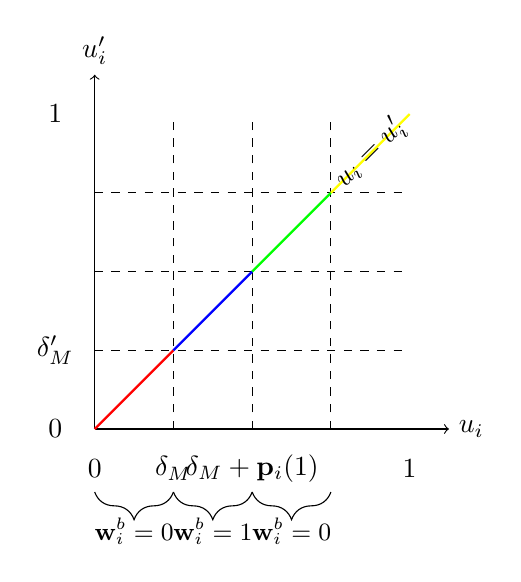
\begin{tikzpicture}
    % Define colors
    \definecolor{myred}{RGB}{255,0,0}
    \definecolor{myblue}{RGB}{0,0,255}
    \definecolor{mygreen}{RGB}{0,255,0}
    \definecolor{myyellow}{RGB}{255,255,0}

    % Draw axes
    \draw[->] (0,0) -- (4.5,0) node[right] {$u_i$};
    \draw[->] (0,0) -- (0,4.5) node[above] {$u'_i$};

    % Draw dashed grid lines
    \foreach \x in {1,2,3}
        \draw[dashed] (\x,0) -- (\x,4);
    \foreach \y in {1,2,3}
        \draw[dashed] (0,\y) -- (4,\y);

    % Draw segments
    \draw[myred, thick] (0,0) -- (1,1);
    \draw[myblue, thick] (1,1) -- (2,2);
    \draw[mygreen, thick] (2,2) -- (3,3);
    \draw[myyellow, thick] (3,3) -- (4,4);

    % Draw labels
    \node at (0,-0.5) {$0$};
    \node at (1,-0.5) {$\delta_M$};
    \node at (2,-0.5) {$\delta_M + \mathbf{p}_i(1)$};
    \node at (3,-0.5) {};
    \node at (4,-0.5) {$1$};

    \node at (-0.5,0) {$0$};
    \node at (-0.5,1) {$\delta'_M$};
    \node at (-0.5,2) {};
    \node at (-0.5,3) {};
    \node at (-0.5,4) {$1$};

    % Draw braces and annotations
    \draw[decorate,decoration={brace,amplitude=10pt,mirror}] (0,-0.8) -- (1,-0.8) node[midway,yshift=-0.5cm] {\small $\mathbf{w}_i^b = 0$};
    \draw[decorate,decoration={brace,amplitude=10pt,mirror}] (1,-0.8) -- (2,-0.8) node[midway,yshift=-0.5cm] {\small $\mathbf{w}_i^b = 1$};
    \draw[decorate,decoration={brace,amplitude=10pt,mirror}] (2,-0.8) -- (3,-0.8) node[midway,yshift=-0.5cm] {\small $\mathbf{w}_i^b = 0$};

    % Diagonal label
    \node[rotate=45] at (3.5,3.5) {$u_i = u'_i$};

\end{tikzpicture}

\end{document}